\documentclass[12pt,twoside]{article}

\usepackage[utf8]{inputenc}
\usepackage{template}
\usepackage{lipsum}

\usepackage{apacite}
\bibliographystyle{apacite}

\usepackage{Sweave}
\begin{document}
\Sconcordance{concordance:report.tex:report.Rnw:%
1 10 1 1 0 68 1 1 18 19 1 1 8 15 1 1 17 19 1 1 29 14 0 1 2 1 1 1 22 10 %
1 1 25 10 1 1 9 14 1 1 4 20 0 1 2 13 1}


\begin{titlepage}
\newcommand{\HRule}{\rule{\linewidth}{0.5mm}} 

\center % Center everything on the page

%	TITLE SECTION

\mbox{ }
\vspace{75mm}

%\HRule \\[0.8cm]
{ \Huge \bfseries \color{black}{Analysis of whistler weather data}}\\[0.4cm] 
%\HRule \\[1.5cm]

{\Large
\textsl{Stat 300 Project, Fall 2015}}

\bigskip
{\Large
by Nathan Esau, Ethan Sim, Benjamin Chan}

\vfill

%\vspace{15mm}
%\begin{figure}[!ht]
%\begin{center}
%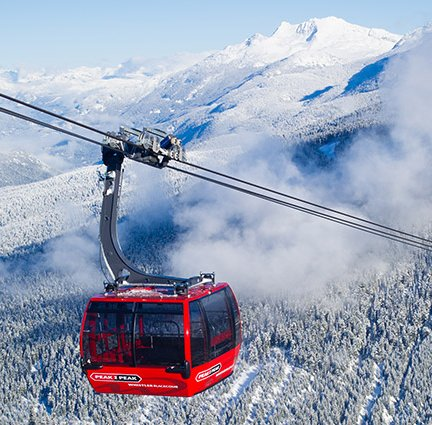
\includegraphics[width=0.9\textwidth]{tp_picture.jpg}
%\end{center}
%\end{figure}

%\vfill
%{\large
%Stat 300 Group Project \\ 
%\medskip
%Fall 2015}

\end{titlepage}

%\thispagestyle{firststyle}
%\noindent
%{\Large \textbf{Analysis of Whistler Weather Data}} 
%
%\medskip\noindent
{%\large \textsl{by Benjamin Chan, Ethan Sim and Nathan Esau}}

\section{Summary}

\subsection{Background}

In this study we analyze daily weather data from Whistler, BC. The variables analyzed were the amount of snow on the ground and the average temperature during each day.

\medskip\noindent
Our study was motivated by trying to answer the following questions:

\begin{enumerate}
\item When is the winter season? When does it start, peak and end?
\item How severe is the winter? How much snow is present at different points in the year? 
\item What trends exist in the data? What odd behaviors have shown up over the past 9 years? 
\end{enumerate}

\subsection{Methods}

\noindent
To answer our questions, we used the following techniques:

\begin{enumerate}
\item Regression, to determine whether there was a trend in the snowfall data
\item Time series techniques, such as average smoothing, to compare different winter seasons
\item Correlation, to determine how different variables were related
\end{enumerate}

\subsection{Results}

\noindent We found that while temperature is very consistent year to year, the amount of snowfall has been showing a downward trend. In particular, the 2009--2010 winter in which Vancouver hosted the Olympics was far less severe, both in the amount of snow and the duration of snowfall, than typical winter seasons. This was shown by comparing the length, average snowfall and peak snow amount of the 2009--2010 winter to other winters.

By averaging different annual time series, we determined what a typical winter season is like in Whistler. In order to do so, we needed to make an assumption about what constitutes the start and end of winter. We classified winter as the period when the average snow on the ground over a week stayed above a given threshold. This contrasts the typical definition of winter as the period from December 21 to March 21.

We also analyzed whether cold winters also tend to have a lot of snow. While these variables do exhibit some negative correlation, we do not have too much evidence that this is necessarily the case.

\subsection{Interpretation}

Whistler weather typically ranges from $\dots$

\section{Introduction}

Whistler Blackcomb is a Canadian resort town in the province of British Columbia, one of the largest ski resorts in North America. Whistler’s economy is highly dependent on the seasonality of snow as the main winter activities offered there are skiing and snowboarding. In July 2003, Whistler was selected to host the alpine skiing events for the 2010 Winter Olympics. However, 2010 was accompanied with an unusually mild winter. The lack of snow made it challenging to run some of the Winter Olympic activities. Given this kind of uncertainty, it would be helpful to have a rough estimate of the when the whistler winter season usually occurs and the peak time of snowfall.

Our weather data was obtained from \url{http://climate.weather.gc.ca/}. Data was recorded at an elevation of 657.80 metres, a longitude of 122$^{\circ}$57'17.400'' W and a latitude of 50$^{\circ}$ 07'44.001'' N over the period 2006 -- 2014. The data set contained the following variables

\begin{itemize}
\item Temperature -- minimum, maximum and mean temperature during each day
\item Snow on the ground 
\item Total precipitation 
\item Wind speed and direction
\end{itemize}

\medskip\noindent The variables most relevant to answering our questions were the snow on the ground and the temperature. For temperature, we decided to use the mean temperature during each day, as we felt this is the most robust measure. We didn't account for wind, due to the large number of missing and truncated values present, or for precipitation which we felt wasn't related to our question. 

We needed to perform some imputation for our variables. In particular, the snow on the ground during the summer months was not recorded, so we made the assumption that these was no snow on the ground at this point. Also, during the winter period when snow was not recorded we imputed the snow value from the previous day. Similarly, when the temperature was not recorded we imputed the temperature value from the previous day. During the winter, there was a small amount of missing values for these variables ($<5\%$) so this imputation shouldn't have a large impact on our analysis.

Our overall goal was to understand the time series shown in Figure \ref{fig:basicts}. In this figure we have shown the two-week moving average for the amount of snow on the ground and the three-week moving average for the mean temperature.


\begin{figure}[!ht]
\begin{center}
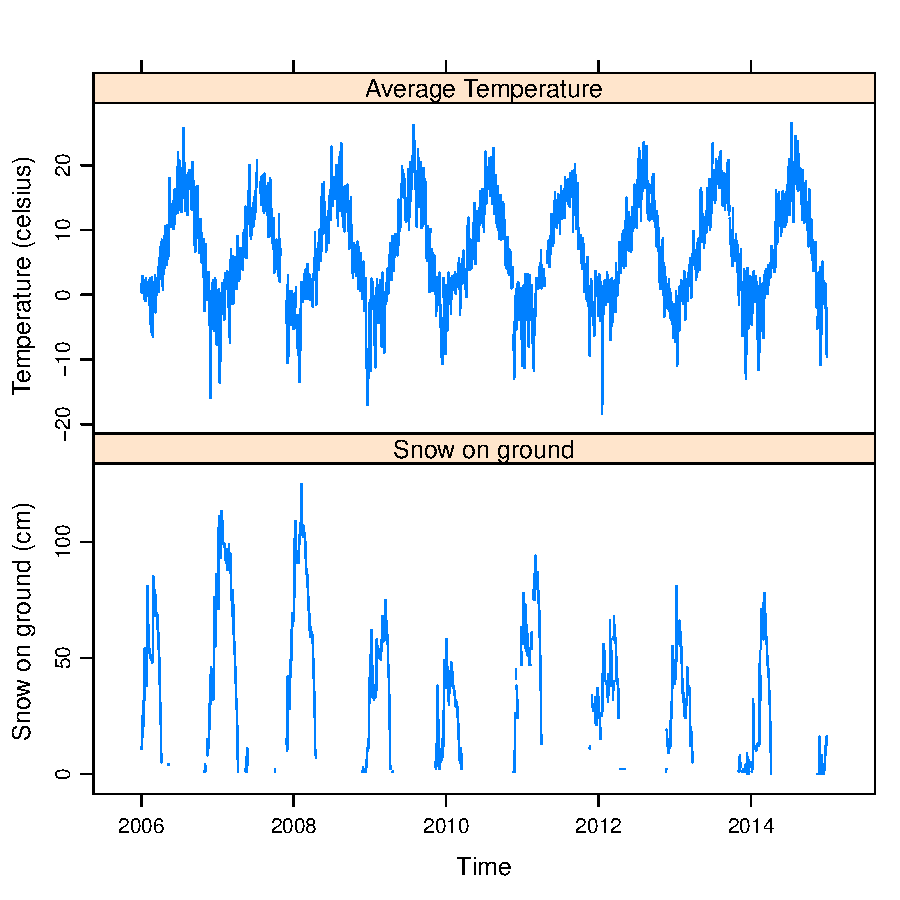
\includegraphics[width=0.8\textwidth]{report-basicts}
\end{center}
\caption{Whistler weather data from 2006 -- 2014}
\label{fig:basicts}
\end{figure}

\section{Methods}

Our methods are divided into the following sections. First, we analyze whether a downward trend exists in the amount of snow during our observation period. Second, we average the annual time series and to determine the minimum, maximum and average amount of snow present in Whistler at each day during the year. Finally, we compare the length and severity of each of the winter seasons. For the severity, we look at the average amount of snow and average temperature during the winter, and analyze whether these results are correlated in some way.

\subsection{Trend}

The trend for snowfall is shown in Figure \ref{fig:snowtrend}.


\begin{figure}[!ht]
\begin{center}
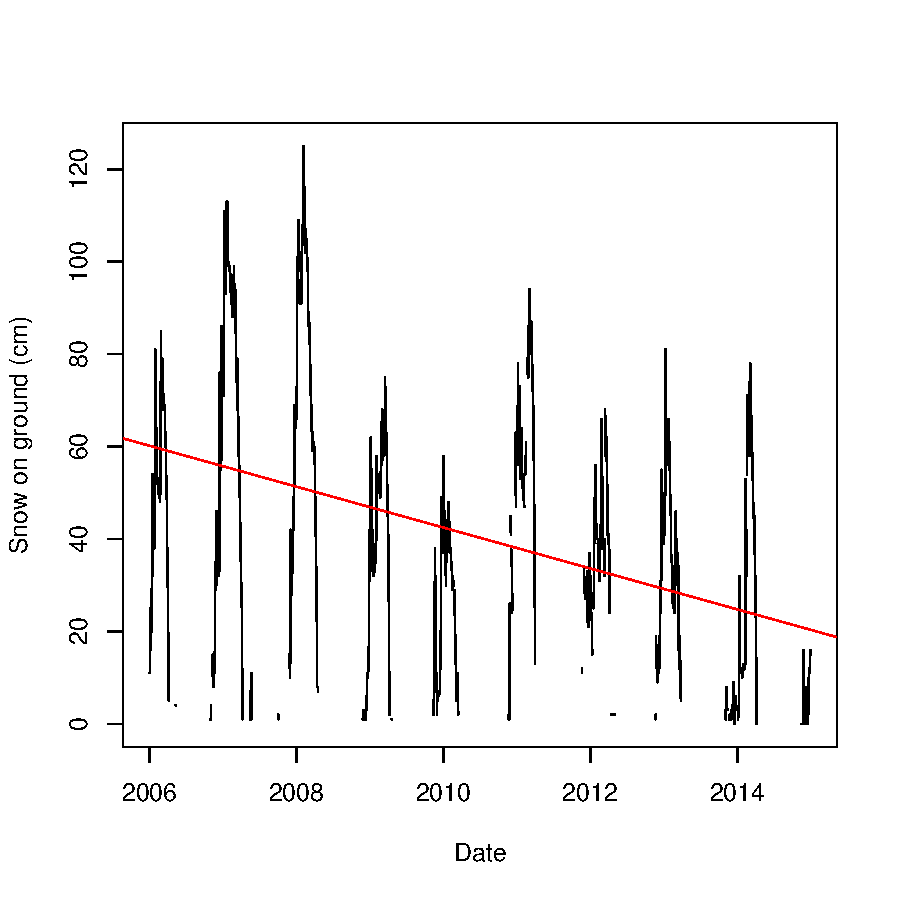
\includegraphics[width=0.7\textwidth]{report-snowtrend}
\end{center}
\caption{Snowfall trend with trend line \textsl{Snow} = 219.4922 -- 0.0121 $\times$ \textsl{Date}. The slope coefficient is significant with $p$-value $<$ 0.001.}
\label{fig:snowtrend}
\end{figure}

The average time series are shown in Figure \ref{fig:averagetsplot}. \lipsum[3]


\begin{figure}[!ht]
\begin{center}
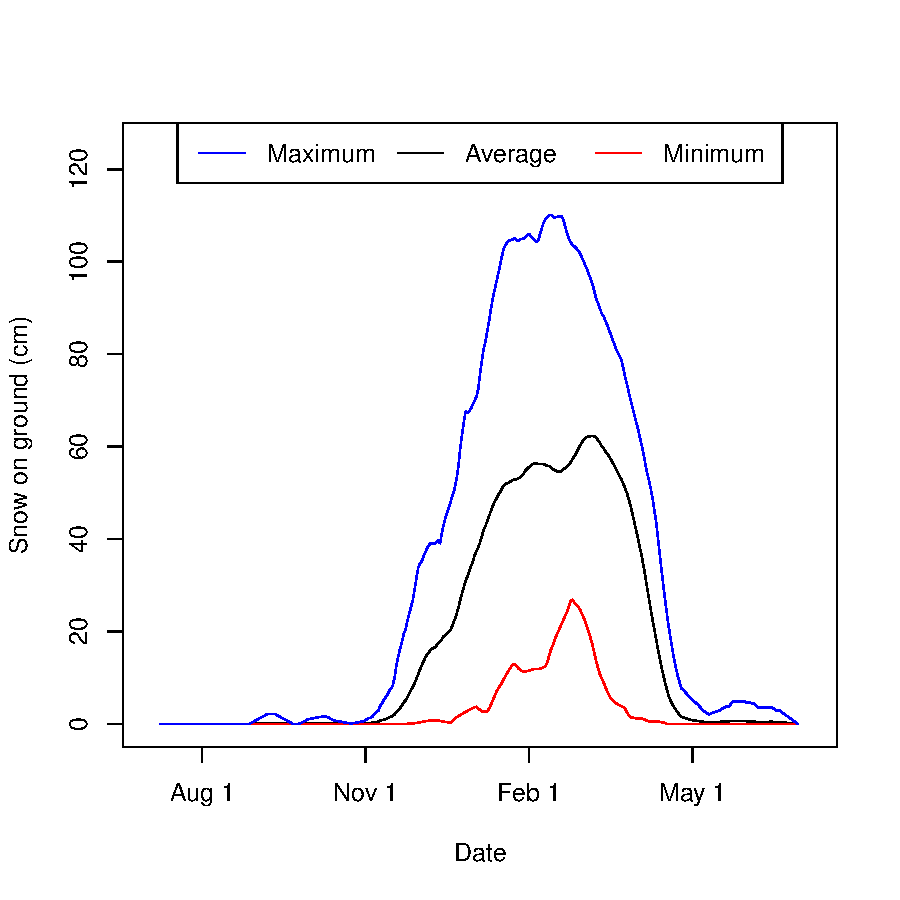
\includegraphics[width=0.7\textwidth]{report-averagetsplot}
\end{center}
\caption{Average, min, max}
\label{fig:averagetsplot}
\end{figure}

The length of winter is shown in Figure \ref{fig:lengthwinter}. \lipsum[4]


\begin{figure}[!ht]
\begin{center}
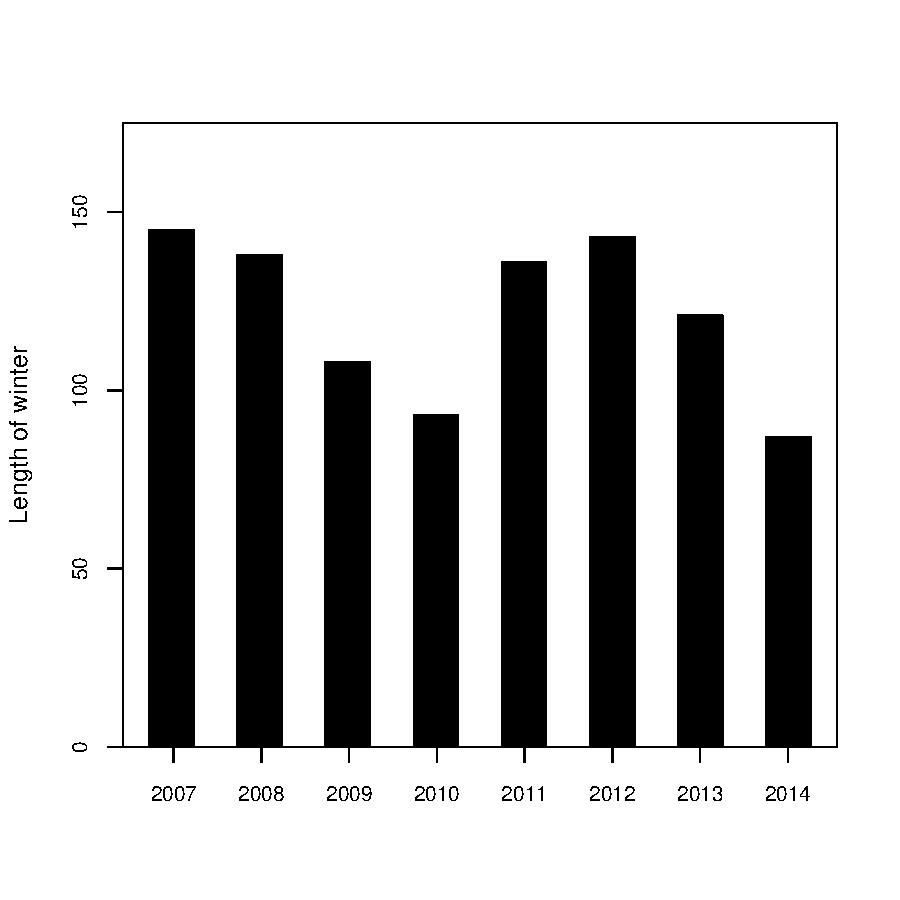
\includegraphics[width=0.7\textwidth]{report-lengthwinter}
\end{center}
\caption{Length of whistler winter season 2006--2014}
\label{fig:lengthwinter}
\end{figure}

The average snow is shown in Figure \ref{fig:averagesnow}. \lipsum[5]


\begin{figure}[!ht]
\begin{center}
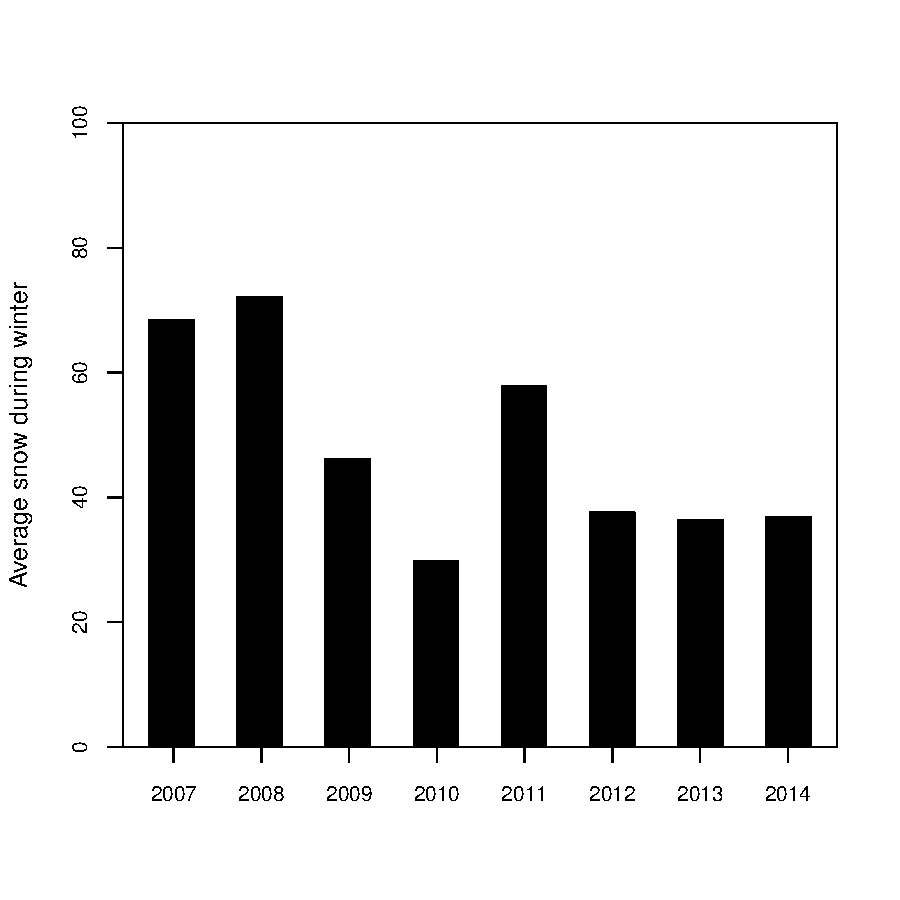
\includegraphics[width=0.7\textwidth]{report-averagesnow}
\end{center}
\caption{Length of winter}
\label{fig:averagesnow}
\end{figure}

The average temperature is shown in Figure \ref{fig:averagetemp}. \lipsum[6]



\begin{figure}[!ht]
\begin{center}
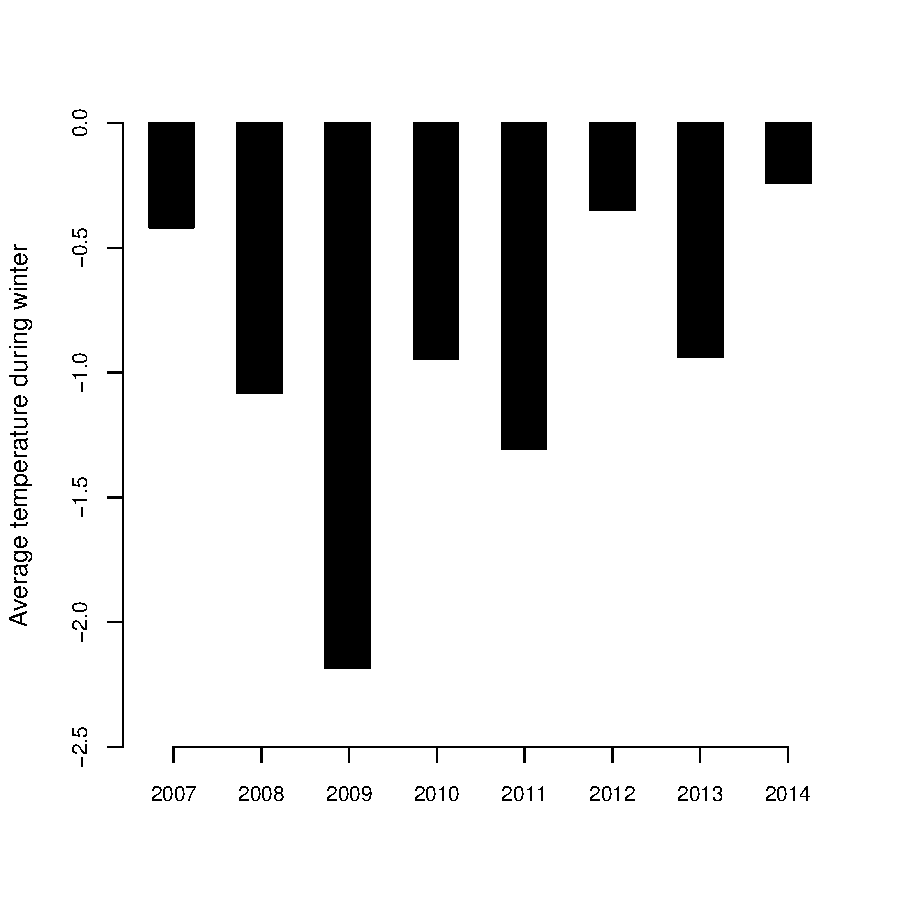
\includegraphics[width=0.7\textwidth]{report-averagetemp}
\end{center}
\caption{Length of winter}
\label{fig:averagetemp}
\end{figure}

\section{Results}

The summary table is shown in Table \ref{summarytable}. 
\lipsum[7].

% latex table generated in R 3.2.2 by xtable 1.8-0 package
% Fri Nov 27 13:20:25 2015
\begin{table}[ht]
\centering
\begin{tabular}{llllrr}
  \hline
Winter & Start & End & Peak & Length & Peak.Amount \\ 
  \hline
2006-2007 & Nov 11 & Apr 5 & Jan 19 & 145.00 & 113.00 \\ 
  2007-2008 & Nov 26 & Apr 13 & Feb 7 & 139.00 & 125.00 \\ 
  2008-2009 & Dec 18 & Apr 5 & Mar 17 & 108.00 & 75.00 \\ 
  2009-2010 & Nov 13 & Feb 14 & Jan 2 & 93.00 & 58.00 \\ 
  2010-2011 & Nov 22 & Apr 7 & Mar 5 & 136.00 & 94.00 \\ 
  2011-2012 & Nov 19 & Apr 11 & Mar 15 & 144.00 & 68.00 \\ 
  2012-2013 & Nov 21 & Mar 22 & Jan 9 & 121.00 & 81.00 \\ 
  2013-2014 & Jan 6 & Apr 3 & Mar 6 & 87.00 & 78.00 \\ 
  Average & Nov 28 & Mar 29 & Feb 12 & 122.00 & 86.00 \\ 
   \hline
\end{tabular}
\caption{Dates table} 
\label{summarytable}
\end{table}
\lipsum

\section{Conclusion}

\lipsum

% To do: COR table

\cite{Williams_1997} and \cite{Andrews_2007}

\bibliography{sources}

\end{document}
